\chapter{Awful}

\section{A Constructed Image}

\keywords{superficial impressions, bitterness, false expectations}

\noindent -- Hello, how are you feeling today?\\
-- Awful.

This is not what a meditator is supposed to say, is it? They should
respond positively, such as, `I'm feeling great, it's such a lovely
day!' Or at least `I'm OK, and how are you?' We have an image of a
`meditator' in our heads who is supposed to behave and speak in certain
ways, while not behaving and speaking in certain other ways. We might
ask, `Who has put that image in \emph{my} head?'

The image of the `good meditator' is a perception formed from
superficial impressions which, without deeper examination, we have
allowed ourselves to see as real. Imagine opening an article about
meditation. (While continuing to read the current one\ldots)

It starts with the smiling photo of a monk or a lay meditation teacher,
and it continues by describing the positive effects of mindfulness. It
might include stories and photos taken at a retreat. People are sitting
on meditation cushions with serene faces while the light through the
window is illuminating the Buddha statue. The article might contain
interview excerpts about how participants had overcome their inner
struggles. It ends with the encouraging words of a meditation teacher,
or with a quote from the Buddha. THE END.

Even someone not terribly interested in meditation knows what this
article looks like, we have seen dozens of them. There is no need to
include a reference source, the chapters in this book could be examples
as well.

This is not to suggest they are being deceitful. The authors write with
good intentions. They are trying to encourage us to continue on the path
of contemplation and to put effort into our practice. If we can't see a
greater happiness beyond the frustrations, what would be the point? If
there was only suffering and misery to expect, we don't need help in
creating that.

\keywords{happiness, get out of your own way, removing blocks from a river, vipassana-glamour}

Buddhism is fundamentally optimistic, and one of its central theme is
happiness. Our typical attitude is that we seek the things which give us
happiness, or that want to create the circumstances necessary for our
happiness. But it is not sure that we understand the right attitude, and
we can become so entangled in seeking happiness, that we become more and
more bitter, as it can seem that such happiness can never be realized.
We assume the fault is in our circumstances or personal abilities, but
in reality the problem is that we don't understand how things work, and
this is why our attitude leads us in the wrong direction.

Our task is not to search for happiness, but to understand the cause
which gives rise to suffering, and stop creating it. Through
understanding this, happiness spontaneously appears in the mind.

Our way of thinking is like continuing to keep carving a statue until it
is \emph{just right}, but with which we are never satisfied. We think
it's our fault, and we don't notice that the materials of the statue are
just the way they are. The clay, sand and stone will remain what they
are. The groups of \emph{khandhas} -- form, feeling, perception, mental
conditions, and consciousness -- will remain as they are. What creates
the struggle is when we expect them to be otherwise.

Effort is necessary, but a more useful metaphor for wise practice could
be that of a choked up river: when boulders of stone are obstructing the
flow of the water, creating turbulence. We tend to focus on the
turbulences of our feelings, and while trying to stop the vortices, we
create more of them. It may be the case that all it needed was to remove
the boulder blocking the flow: grasping the whole thing as `I am this'.
Sometimes we just need to get out of or own way.

If you observe the water flow in a river channel, you'll notice vortices
forming behind obstacles. Their back-and-forth motion might seem
familiar (see Figure \ref{fig-grasping-turbulence}). When holding onto
the perspective of `I am' dominates the mind, we start flipping
back-and-forth between opposites. We reason with ourselves what to do
because `I like A', or `I don't like B', `I should do X', `I shouldn't
do Y'.

Not satisfied with either, but holding onto an identity, the mind is
stuck in a flip-flop between the extremes. One opposite invites the
other as a reaction, the extreme positions being easier to reach, rather
than a cool-headed look at the situation from an outside perspective.

The teachings do mention suffering frequently, but such instruction is
given on the ground that freedom from that suffering is possible. The
Buddha made it clear that the fruit of the path is genuine happiness,
and if it was not possible to practise it, i.e. to abandon unwholesome
roots and develop the wholesome ones, he would not have taught
it.\footnote{\href{https://suttacentral.net/an2.11-20/en/thanissaro}{AN
  2.19}, Skillful}

Who is that meditator in our head? One thing is sure, the one in
\emph{my head} is always a \emph{better meditator} than I am. When
someone takes a good photo of us, we know how it is: it was a good
moment when we looked orderly or even glamorous, but we know that in
five minutes the opposite could be true. And although this is true not
just for us, somehow we don't remember this about good photos taken of
other people.

These are a sort of \emph{vipassana}-glamour shots -- it's a bit vain
but we like looking at them. They make good illustrations in an article,
but we should remember that the same people will look different in an
ordinary moment.

\vfill

\begin{figure}[h]
\caption{Grasping and Turbulence in the Mind}\label{fig-grasping-turbulence}
\hspace*{-9mm}%
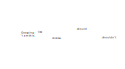
\includegraphics[width=\linewidth+18mm]{./manuscript/tex/diagrams/grasping-turbulence.pdf}

\smallskip

{\footnotesize
Turbulence in obstructed water flow.
The formation of vortices is similar to how grasping 'I am' in the mind
causes one to be stuck in a back-and-forth motion between opposite positions.
Fluid simulation by Amanda Ghassaei (\href{http://apps.amandaghassaei.com/VortexShedding/}{apps.amandaghassaei.com}).
\par}
\end{figure}

\clearpage

\section{Threads}

\keywords{suttas as literature}

\noindent In the days of the Buddha, one form of literature was the
\emph{sutta}, which means a thread of discourse. \emph{Suttas} may
include prose and verse, and were intended to be memorized through
recitation. The community of monks would compose a \emph{sutta} after a
significant event, such as a discussion or formal a teaching, to give
the story a formal presentation in which they would memorize it. The
Buddha certainly encouraged them to do so:

\begin{quote}
Thus you should train yourselves: `We will listen when discourses that
are words of the Tathāgata---deep, deep in their meaning, transcendent,
connected with emptiness---are being recited. We will lend ear, will set
our hearts on knowing them, will regard these teachings as worth
grasping \& mastering.'

\bigskip

\quoteRef{%

\href{https://www.dhammatalks.org/suttas/SN/SN20_7.html}{SN 20.7}, The
Peg

}
\end{quote}

Today, books, articles and blog posts fulfil a similar function, to
distribute curated information. These modern media, when bringing their
best form, hold up the canonical \emph{suttas} as their example. The
monks of the early years delivered their message to us through these
threads, and their efforts have become part of our conversation with
those we meet today, just as our written works will speak to those in
the future who we will never meet.

\clearpage

\keywords{social media, selection bias, Instagram Effect}

In today's social media the clear understanding of the message is
distorted by what is called `the Instagram effect', which is a selection
bias to show only our best and most positive side, and filter out the
negative one, which is nonetheless just as real and necessary for
complete understanding.

This influence is not negligible. Medical studies have already started
discussing a related form of depression and obsessive behaviour called
`Snapchat Dysmorphia'.\footnote{\href{https://www.ncbi.nlm.nih.gov/pmc/articles/PMC5933578/}{Is
  ``Snapchat Dysmorphia'' a Real Issue? (ncbi.nlm.nih.gov)}} In these
cases a given person seeks cosmetic surgery to look more like the
smiling photos they see in the application.

The automatic filters of the app edit every picture to be more
attractive, and if we repeatedly see our bodies shown to us (by the
application) as a nearly flawless image, \emph{that} becomes our mental
self-image, and the unfiltered image we see in the mirror seems wrong to
us.

One might consider a similar Instagram Effect in published articles
about meditation experiences. The author has a point to explain, and
they select a mix of personal experiences, opinions, and supporting
explanations from other authors.

The author may write truthfully and try to avoid selection bias, but
subtle, unconscious forms of self-filtering keep operating. The world of
the written text is always a constructed reality. Nonetheless, when it
succeeds in its goal, in the well-chosen words we recognize our own
experience.

\clearpage

\keywords{our mental images as role models}

The meditator who lives in our head is like a character in a poem, or
the hero in a myth. Our heroes are wiser and stronger than we are, so
that when we are feeling lost and weak, they can give us faith and
advice. They can have unshakeable peace, so that when we are feeling
awful, we are able to endure and wait until the difficulty ends.

Such mental images are, however, just that, and shouldn't be mistaken
for a real person. They are valuable sources for guiding ourselves,
their narrative description helps us to figure out what to do by showing
where we are in a bigger picture.

The role of a mental image is not to determine what we \emph{should
become}. When we relate to perceptions and ideals like that, we are
going to feel conflicted and inadequate, because the real circumstances
of our life are far more complex, rich with ambiguous, shifting
boundaries, and are not like the simplified, static reality of a mental
image. Mental images are tools for explanation. They are \emph{ways of
seeing} the world, and are examples of acting correctly in a given type
of world.

\clearpage

\section{Assumptions}

\keywords{mind and the world, mode of attention, actions and beliefs}

\noindent We may remember the verse in the Dhammapada which points out
that the world of our experiences is not independent of us:

\begin{quote}
Mind precedes all states of being: they are led by the mind, made by the
mind.

\emph{Manopubbaṅgamā dhammā, manoseṭṭhā, manomayā.}

\bigskip

\quoteRef{%

\href{https://suttacentral.net/dhp1-20/pli/ms}{Dhp 1}

}
\end{quote}

Does that mean that we are creating imaginary problems for ourselves?

We may start investigating by asking, `Can the subject experience
suffering?' Living beings can suffer, but a cultural idea or self-made
story cannot suffer, even while \emph{we are}. It changes our attitude
if the subject of our concern only exists as a story and not as a living
being. Such insentient stories include the narratives we have around
institutions, nations, money, fame, or other social fabrications.

Next, a quick moral safety test: `Would a wise person praise or
criticize doing this?'

Further on, bringing our view to the surface: `What assumption creates
this stress and pressure? What is the motivation for doing this? Without
what, would this have no significance?'

We can reveal such unconscious motivations by looking at our present
actions and choices. What we choose to do now expresses what we believe
in, the assumptions we have accepted in the past.

`Why am I choosing to do this, here? Where does this action come from
and where does it lead?'

The underlying factors for our actions may come, for example, from the
habitual conditioning of our environment. We may have not expressed in
thought why we do what we do, but have felt \emph{the results being
expressed on us}, whether good or bad.

Starting the investigation with a closer look at our actions and
\emph{then} asking about the thoughts motivating them is a productive
method. In our inner chit-chat we tell all sorts of contradictory things
to ourselves, but our actions give clear points of reference.

\keywords{the best place to learn, reversing assumptions}

The associated feeling might be awful, but if we treat it as sign to
turn toward the mind and investigate it, our approach will stay
practical and productive. `If I am here anyway, what can I learn from
this?'

We find access to our assumptions through uncovering our unconscious
motivations. Once we can express an assumption clearly, we gain the
freedom to reverse it, or drop it.

We may ask, `Does it help in this situation, if I reverse my
assumptions?' Perhaps looking at it in the opposite way is exactly what
is we needed either for peace of mind, or for dropping the issue as if
it never existed. Either way, we are not acting out of compulsion: we
are free to either let it go or \emph{choose} to follow it through.

\clearpage

\section{After the Storm}

\keywords{happiness and accomplishments}

\noindent Meditation guides say, `return to the present moment', but it
doesn't mean that you must like everything you find there. The point is
that this is the only place where you can live. If you are happy, you
are not happy in the future, but in the present. If you are suffering,
you can't understand it in the future, only in the present. In some
situations, no amount of brainy self-talk is going to make it better, it
is best to call it the way it is, and wait out the storm like a stoic.
Conflict is genuinely stressful, separation from what we love is sad,
and being alive always ends with the tragedy of our own death.

We tend to anticipate success, and we expect our hard work to be
justified in the future. Examine that moment of accomplishment, what do
you experience? There may be some emotional elevation -- surprise, joy,
exhilaration, relief -- then everything is back to the ordinary level.
The destination turns out not to be the deliverance we thought it would
be. If we were intensely focused to get there, we might not even
remember anything from the journey, and wonder where did all the time
go. We can be so intent on being productive, that we waste our chance to
live.

Contemplating death holds up a truthful, if somewhat scary, mirror to
our values. `If I were to die tonight, would I be happy to remember
living as I am living today?' This question can stir up more from the
deep recesses of the psyche than we wish for. I remember a time when my
response the word `happy' was exclusively anger and self-aversion.

\clearpage

\keywords{values, being busy, Hedonic Treadmill, burnout, contentment}

The term `Hedonic Treadmill' describes the adaptive process in which
each new achievement becomes the new norm in our psyche, and we feel
less and less emotional impact after succeeding at our goals. Like on a
treadmill, no matter how hard one tries to increase one's happiness by
pushing toward the next successful step, one still remains in the same
place. We spend our life travelling on the journey, not hanging out in
the destination. If we look closer, even the idea of any destination
evaporates, like when you fly into a cloud. `I thought I saw it right
ahead, but now that I'm here, I can't see it.'

Despite this, we seem to continue thinking that being busy, productive
and efficient, is somehow going to save us. When one project is
finished, we can feel that we \emph{need} another one because being busy
is the only way of existence we know.

\enlargethispage*{2\baselineskip}

The wise men of old repeat their message about contentment, but it seems
that we have to suffer the pain of burnout before we comprehend what the
problem is.

Bertrand Russell gives a diagnoses, `One of the symptoms of an
approaching nervous breakdown is the belief that one's work is terribly
important.'\footnote{\href{https://www.goodreads.com/book/show/51783.The_Conquest_of_Happiness}{The
  Conquest of Happiness by Bertrand Russell}} Henry D. Thoreau writes in
his cabin by Walden Pond, `It is hard to have a Southern overseer; it is
worse to have a Northern one; but worst of all when you are the
slave-driver of yourself.'\footnote{\href{https://www.goodreads.com/book/show/16902.Walden}{Walden
  by Henry David Thoreau}}

\clearpage
\figurepagelayout

\begin{figure}[h]
\caption{Achievements and the Hedonic Tredmill}\label{fig-hedonic-treadmill}

\centering

\includegraphics[width=90mm]{./manuscript/tex/diagrams/hedonic-treadmill-stairs.pdf}

\bigskip

\begin{minipage}{0.8\linewidth}
\centering\footnotesize

The Hedonic Treadmill is the tendency for new achievements to be adopted as a modified, \emph{normal} baseline,
and for our level of happiness to return to the same level as before.
After one desire is satisfied, the conditioned craving seeks a new state.

\bigskip

The person on the Penrose Stairs thinks that
they are getting further and higher.
From our outside perspective,
we see that they are merely returning to the same level as before.

\bigskip

Recall the definition of Noble Truth of the Origin of Suffering:
`It is this craving which leads to renewed existence,
 accompanied by delight and lust, seeking delight here and there;
 that is, craving for sensual pleasures, craving for existence,
 craving for extermination.'
(\href{https://suttacentral.net/sn56.11/en/bodhi}{SN 56.11})

\end{minipage}

\end{figure}

\clearpage
\normalpagelayout

What if you practice \emph{being free}, instead of practising \emph{to
become free}? The system of gradual training described by the Buddha --
while encouraging us to make diligent effort in our practice -- starts
with blameless happiness in the present, born of contentment through
moral- and sense-restraint.

\begin{quote}
{[}\ldots{]} they practice restraint, protecting the faculty of mind,
and achieving its restraint. When they have this noble sense restraint,
they experience an unsullied bliss inside themselves.

\bigskip

\quoteRef{%

\href{https://suttacentral.net/mn38}{MN 38}, The Longer Discourse on the
Ending of Craving

}
\end{quote}

\keywords{self-aversion, self-criticism, labyrinth of mirrors}

It is easy to over-correct being busy, and swing to the other extreme:
`I've had enough! I'm just going to quit everything!' This might seem
``logical'' but, being driven by aversion, we continue to suffer. For
many of us, it is easy to be critical of ourselves, and we diligently
practice it with conviction to prove ourselves wrong, as if
self-aversion was a virtue.

`I am feeling awful! A \emph{real} meditator would never feel like this.
I must be doing something wrong.' A whole identity can be built around
this, a ceaseless internal monologue which always responds with
complaints and self-aversion. One can live like this for decades, and it
becomes the baseline by which we recognize ourself. `If I wasn't feeling
angry, I wouldn't even know who I was.'

It is like being stuck in a labyrinth of mirrors: everywhere you look,
you only see yourself. The key to escape is to find a crack in the
mirrors, and recognize change: the feelings of being driven, and the
motivations of anxiety and anger which we thought were constant are, in
reality, changing all the time -- breaking up and reforming. This
labyrinth has been made by the mind, and what it has created is empty of
self. It cannot be what we truly are.

Doubtless, we can find a persuasive logic in our self-defeating
ideations, and our reasoning for being critical can be completely
reasonable! Psychologists say that the most difficult patients are the
ones who intelligently defend and justify their own bad habits. We can
be so clever that there is absolutely no way to be happy \ldots{} and we
can prove it! Can you recall ever playing the role of such a miserable
philosopher?

But we do not necessarily experience immediate relief when our
self-reflection reveals to us the emptiness of what we have been
pursuing. Anger, despair\footnote{The Buddha compares dealing with anger
  and despair to walking along a path close to a deep drop-off.
  (\href{https://suttacentral.net/sn22.84}{SN 22.84}, With Tissa)} and
sadness can be our first reaction, generating thoughts of self-aversion.
We purify the mind with the mind: These mind states are not reliable,
they shut down our intelligence, and who wants that? So we let go.

\keywords{patient endurance, gratitude, no hurry}

Patient endurance is an underappreciated virtue, but often, all we need
is to remember to wait: the dramatic rain and thunder of turbulent
mental states will run themselves out.

When the sense of gratitude appears, it is a sign like the rainbow after
a storm. It accompanies wholesome mental states, and we can
intelligently see the situation from more than one angle. This is a good
base from which we can build useful thoughts about what to do next.
Sometimes, the best thing to do is to simplify and turn away from
certain habits and values. Other times, our view has changed and we
might wish to keep up what we have been doing, but leaving the big hurry
behind. We continue for the sake of living it, not waiting for some kind
of elevated mental state in the future.

\begin{quote}
One should not revive the past\\
Nor speculate on what's to come;\\
The past is left behind,\\
The future is unrealized.

\bigskip

\quoteRef{%

\href{https://suttacentral.net/mn131}{MN 131}, One Fine Night

}
\end{quote}

\section{Humour and Irony}

\keywords{opinions, changing perspectives, noticing what is pleasant}

\noindent There are morose, dark moods which are like sand-traps of
logic, made by ourselves. The more we think about them, the deeper we
sink in them.

Humour and irony are funny because they show the situation from
unexpected and odd angles. If the logical path straight ahead is
blocked, why not try the sideways track where the fox goes? A joke
wouldn't be funny if it was logical and reasonable. Humour and irony,
directed toward ourselves, are good friends when it seems that we can't
escape the suffering of our thoughts.

What makes the old and wise men \emph{wise}? Medical studies\footnote{\href{https://www.researchgate.net/publication/258190619_Aging_irony_and_wisdom_On_the_narrative_psychology_of_later_life}{Aging,
  irony, and wisdom, William Randall (researchgate.net)}} have
investigated the various attitudes of senior citizens, and found that an
inclination toward self-directed humour and irony (i.e. being able to
laugh at oneself) was helpful to face the significant challenges of
ageing and maintain mental balance and a positive outlook on life.

One of their key observations is that humour and irony develop our
ability to see ourselves from multiple viewpoints. We can fill the role
of the accurate historian and the jesting comedian at the same time.
Hence we are able to see events from multiple narrative angles and not
be caught in a single story. The frame of the narrative we see ourselves
in remains open as we move toward a positive future. The limits of our
being don't necessarily mean the end of the story, and we don't have to
go far to find good laugh: in the absurd corners of life, there is
always a joke to tell.

It can be rude to joke about somebody else's bad situation, but who is
going to get upset over your humorous comments about yourself? If you
feel awful, how about an awful joke? This trip is so bad that it's good,
and the tickets are free. `What am I? An animated skeleton in a skin-bag
with clothes on, standing here with a fabulous hair-cut, and I can prove
the logic of \emph{my important} opinions.' What's not to laugh at?

\enlargethispage*{\baselineskip}

We say that in meditation we observe our own mental habits, but
sometimes we practise this with a critical bias: we observe the
\emph{bad mental habits}, while we don't notice the good ones. It is
possible to become so good at ignoring pleasant mind states that one
genuinely believes happiness only exists for other people. When
something good happens and you feel happy, stop and notice it, `Hey,
this is nice.' This increases our capacity to recognize and experience
such mental states in the future. Who will notice it if you don't?

\section{Expectations}

\keywords{symbol of Buddha statues, changing predictions, relinquishment}

\noindent We might look at a Buddha statue and expect ourself to
meditate in the same perfect posture without moving, like the Buddha.
But in this case we have missed the message of the statue, which points
to inner qualities rather than external signs.

A Buddha statue is not a depiction of the historical \emph{Siddhattha
Gotama} Buddha who lived in the 5th century BC. We don't have a statue
of him made during his lifetime. We know from the \emph{suttas} that he
was normal height and good-looking, but instructed the monks to not
focus on his physical appearance, bot on the Dhamma, the truths of the
mind instead.

He taught them that even if a monk were grabbing hold of the corner of
his robe, but if they didn't see the Dhamma, they would not see the
Buddha.\footnote{\href{https://suttacentral.net/iti92}{Iti 92}, The
  Corner of the Cloak} The first Buddha statues were made four or five
hundred years after his death by Greeks in the Gandhara region of
Afghanistan. Buddha statues represent the wisdom and serenity of the
awakened mind, expressed in the human form.

They are beautiful to look at, but nobody is going to become a Buddha
statue, just like you can't become the photo of the perfect meditator,
or the hero in lyric poem. They do offer advice, but the advice can't
orient us when taken rigidly. We should apply the advice by taking our
inner experience and the present situation into account. This way we
return to the awareness which awakens to the truth and overcomes
obstacles. The practice of virtue, and the trust in the examples of
skilful teachers is a strong foundation. We can wish ourselves well,
while still admitting that we feel awful, when that's how it is.

Expectations are a prediction of the expected value of a result, they
estimate the outcome of our situation. Meanwhile, every factor which
goes into that prediction is changing. We have to allow the prediction
to change, our expectations of our mental experience must keep changing
according to where we are now. Having expectations is not a problem, but
if we attach to a particular outcome which we believe to be `the real
one', this becomes a hindrance. It turns out that if we invest in future
emotional states as the basis for our happiness, the result will be
disappointment.

\enlargethispage*{\baselineskip}

The \emph{ānāpānasati} breathing technique taught by the Buddha has
sixteen steps. The first is knowing whether the breath is long or short.
But what is the last step? We might wonder, `What could be that exalted
mind state which we will reach?' Mindfulness meditation on the
breathing, after contemplation of the body, feelings, and mental states,
follows contemplating the natural truths, of which the last step is:

\begin{quote}
One trains thus: `I shall breathe in contemplating relinquishment'. One
trains thus: `I shall breathe out contemplating relinquishment'.

\bigskip

\quoteRef{%

\href{https://suttacentral.net/mn118}{MN 118}, Mindfulness of Breathing

}
\end{quote}

The practice of the Eightfold Noble Path is not about accumulating, but
about transforming our values through insight into the experience of
changing conditions. At the end we relinquish the conditions, like
putting down a burden and not carrying it any further. This includes all
that we take to be `me and mine'. Anyway, how long can we really hold
onto anything?

\keywords{real practitioner, Impostor Syndrome}

Reflection and cultivation opens up a wider field of view where
opposites can exist in complex relationships. In the contrasting
approach, we exalt the judgmental and comparing mind, and this limits
our scope. Such a perspective wants to sort things into neat, mutually
exclusive abstract categories, which leads to mistrust and harm. We
start losing faith, not believing ourselves to be `real' practitioners,
and others don't seem to be credible ones either. The result is that we
can't learn from ourselves, and we can't accept anyone to teach us
either. This doubt is blinding and paralysing, it feels like we can't do
anything. The problem is that our expectations are too narrowly focused.

It's not that there are no problems and difficulties. Explaining to
ourselves that `pain is not painful' is not a meditation technique
taught by the Buddha. But we shouldn't assume that we should be like
mythological ideals. Meditation is not a button to control mental
states. It is cultivating awareness, so that mental states don't control
us.

\section{Calibrating Emotions}

\enlargethispage*{\baselineskip}

\keywords{learning emotions, variation is the norm, disappointment, saññā and saṅkhāra}

\noindent When we talk about emotions to each other, we often explain
their mechanism roughly as a `neural circuit', or a region in the brain
which gets activated in a certain situation. According to this story,
some brain areas are wired from birth to produce given emotions, and
they make us feel fear, love, anger or disgust.

But then how do we explain it when a person without an \emph{amygdala}
still experiences fear? The \emph{amygdala} is typically seen
responsible for that emotion.

Or how about more refined categories?

The Japanese `\emph{mono no aware}' means a sadness over transience and
the beauty found in that, are the Japanese born with such a neural
circuit? By the description, you might recognize the feeling, if you
have seen Japanese movies it might even be familiar, and now, fitting a
verbal expression on it, it gets easier and easier to feel it.

Other cultures find the western emotions strange, for example the Utka
Eskimos, who have no direct equivalent of the concept of `anger.' Or the
Tahitians, who have no concept of `sadness.'

Medical research informs us that no particular emotion has a built-in
`brain-circuit' from birth.\footnote{\href{https://www.goodreads.com/book/show/23719305-how-emotions-are-made}{How
  Emotions Are Made: The Secret Life of the Brain by Lisa Feldman
  Barrett}, Theory of Constructed Emotion} It is not the given emotion
that is fundamental, but our ability to recognize patterns of loss and
reward, to \emph{learn emotion concepts} from other people, and to
recognize them in a new situation in the future.

In any given situation, the brain recognizes if an earlier experience
\emph{in a similar context like this} was rewarding or not. This becomes
easier over time if we have learnt to associate an emotion concept with
it, becoming a spontaneously automatic feeling.

The instances of an emotion category are variable: `fear of a tiger' is
different from `fear of an exam', which are learned and adaptive
predictions. They fit only to some extent, like a person may fit a
stereotype, but no person is a 100\% example of every feature of the
stereotype.

Our brain evaluates the present based on the past, and according to
whether good or bad can be expected, there is a response we feel
throughout the body, and we construct an instance an emotion from it
based on our concepts.

\keywords{emotions are categories, not distinct mental object, learning emotions, what is wrong with me}

In the classical model of emotion -- which we are accustomed to in
everyday discussion -- we treat emotions as distinct mental objects. The
idea is that an emotion has clear attributes that any two mentally
healthy people should agree on.

However, while they were studying the brain in action, it became
apparent to the scientists that this cannot be the case. As they
conducted more and more studies, the evidence continued to contradict
this view.

When people undertook physical and psychological tests about the
emotions they experienced, the results had great variation between
individuals. There were no universally distinct, clear markers, or
`fingerprints' to identify any given emotion. Rather, the
\emph{variation was the norm} in both people's emotional experiences,
the meaning and function of those emotions, and their corresponding
physical reactions.

The scientists found that our body and brain \emph{learns} emotion
categories through a process of conditioning perceptions. From our
culture, the other people we live with (socially conditioned emotions);
from biological needs (bodily conditioned \textasciitilde); or from our
personal history, such as long-time habits, significant events and our
memories.

This also relates to how one person might not understand, or not even
recognize, the emotions of another. For example think of the culture
shock when visiting a distant country: an emotion such as `love' has a
variety of expressions, contexts and underlying assumptions which were
not part of our earlier emotion category of `love'. It can take a while
to pick up the new signs and meanings until we can feel the subtle
differences, and we can reliably recognize the signs in others.

Ask yourself, how do you know that you are feeling a particular emotion
such as \emph{metta} (loving-kindness) or \emph{sukha} (happiness)? The
model we use for our understanding of emotions influences what we expect
to happen in our meditation practice. If we think of emotions as
distinct things, as though they were external objects which we wish to
reproduce, or have access to, then we can easily feel `this is not it, I
don't know what's wrong with me'.

Since \emph{variation is the norm}, our experience will probably differ
from other people's. Individual meditation experiences are as varied as
the individuals. A given instance of an emotion can be expected to vary
from the generalized idea. It is important to rely on knowing \emph{our}
mind states and feelings, instead of trying to reproduce external
descriptions.

Our freedom extends to learning and constructing emotions we never heard
of before. We rely on mindfulness to perceive our experience, we
self-train the concept, and establish the conditions for the emotion to
arise.

Using the terms of the Five Khandhas, we would say that perceptions
(\emph{saññā}) and mental conditioning (\emph{saṅkhāra}) influence each
other and establish patterns of experiences, which we learn to identify
as a present instance of a broader, abstract emotion category.

We start with reading the external description and we turn it into an
inner experience through reflection and daily actions. Knowing our
experience is the reference point. Over time, the new experiences become
familiar to us and they arise without effort.

\keywords{emotions as predictions, culture shock, adjusting expectations}

The brain is constantly receiving signals from the nervous system, and
based on what it has learned, it tries to predict whether the present
situation is going to mean energy input or energy expense for the body.

The brain responds by preparing your body, such as increasing or
decreasing the heart rate, starting or stopping the production of
certain hormones. We experience this bodily reaction, and if earlier we
learnt an emotion category which suits this, we feel an instance of that
emotion: fear of danger, excitement in anticipation of immediate reward,
or euphoric happiness.

This explains culture shock: if you have grown up in a different
culture, you've learnt different emotion categories, and when travelling
to a distant country, the emotional world of the people living there can
be unfamiliar to you.

We tend to believe that our experience is like the view when we look out
a window. One `looks onto their experience', and sees what is going on.

It turns out that the picture is rather more incomplete than we think,
when we take into consideration how the senses and the nervous system
work. The brain doesn't have much information to work with, so it has to
guess at what is happening from simple signals, hints about what the
rich world outside of itself might be like.

The brain can't see much: it's sitting in the skull, which is, in
effect, just a dark box. Bodily fluids, chemicals and nerve signals
carry messages into this box. The messages come from other systems in
the body, which are themselves noisy and sometimes conflict with each
other. From this clutter, the brain has to generate a perception of the
place where we are, guess what is happening to us, predict what is
likely to happen in the next minute or so, and produce a response which
is hopefully going to help us survive, or even lead to happiness. It has
to do all this, from inside a dark box, based on a few noisy and limited
signals.

\clearpage

What am I then? An animated skeleton, and my head is a dark box? Well,
that does explain a lot of confusion. Is it a wonder that my predictions
are a bit off, and need constant adjusting? What I experience as reality
is ongoing guesswork, changing by the second.

`Happiness equals reality minus expectations' -- a memorable phrase by
Tom Magliozzi. These days, our expectations are so high. We receive
updates from social media apps, we read web articles, and each time they
influence our view of how we are, and how the world is around us. They
show us perfect, determined, or outrageous images of other people. Since
we don't meet these people face-to-face, we don't see the real
background of their lives, and this exaggerates our expectations. It
trains the brain again and again to expect these artificial
presentations, like an expectation machine on overdrive. We don't even
notice the distorted self-conditioning, but we are disappointed and
exhausted, which leads to ceaseless dissatisfaction.

\keywords{simplicity, impermanence, self-reflection, values}

We have the ability to calibrate the `expectation machine' through the
balancing effect of conscious reflection and reasoning. `What is the
most important today? What do I need for this one day?' When you
simplify the answer down to the essentials, it's not that much. Food,
clothes, shelter, medicine, supportive companions and perhaps something
to do toward a worthwhile goal.

The average day is probably more messy, and doesn't hold to this
abstract, pure simplicity, but this exercise is only for recognizing the
baseline. If simple is enough, then it won't be a problem to be able to
do more, or have access to more, while contentment remains our baseline.
Ambition is not the problem, but hyping up our expectations blocks its
application.

Expectations are necessary to follow a given direction in the world, but
not understanding them, they become obstructions in the heart.
Expectations and emotions are of the nature to arise, twist, flip-flop
and then turn around. Let them pass on by, like leaves in the water next
to a boat. Bad ones are not that bad and good ones are not that sure.
Knowing their changing nature, we don't take them so seriously and don't
get stuck on them, as a boat shouldn't get stuck on some leaves.

\begin{quote}
Whether it be pleasant or painful\\
Along with the neutral,\\
Either internal or external,\\
Whatever feeling there is:\\
Knowing them, `This is suffering,\\
deceitful and disintegrating,'\\
Coming in contact again and again,\\
seeing their fall,\\
One loses one's passion for them.

\bigskip

\quoteRef{%

\href{https://suttacentral.net/sn36.2}{SN 36.2}, Pleasure

}
\end{quote}

\clearpage

\section{Happiness as Flourishing}

\keywords{meanings of happiness, results, day-by-day practice, death, contentment}

\noindent Our modern Western culture often presents happiness as a
particular feeling, or as a certain circumstance in life which we are
supposed to arrive at. We pass on our culture through discussion with
one another. Our way of talking about happiness tends to treat it as an
outcome, as an event in the future, or as a certain state of being. This
seems to be a recently developed trend, and not necessarily a helpful
one.

Traditionally, we view the ancient Greeks as one of the most influential
societies in the formation of our Western values. Aristotle (384-322 BC)
is one of these influential thinkers, and today we are still reading and
referencing his writings which survived the ages. In these texts, he
investigates the question of happiness in great detail.\footnote{\href{https://plato.stanford.edu/entries/aristotle-ethics/}{Aristotle's
  Ethics (plato.stanford.edu)}} He was concerned with what happiness
was, and with how to live a happy life, but, unlike us moderns, he did
not see it as a particular result or circumstance.

The Greek word he used for happiness is \emph{eudaimonia}, and can be
translated as `human flourishing, prosperity.' He saw it manifesting as
a continuously active process which we practice day by day, rather than
an eventual outcome in the future. He describes the practice of
happiness as being based on moral virtue and a truthful view of one's
life from birth, growing up, old age, and including the tragedy of one's
own death.

\enlargethispage*{2\baselineskip}

This direct view of virtue and mortality puts things in order: it gives
us a wide perspective in which happiness is founded in wholesome mental
qualities, and we look beyond ourselves to give lasting meaning to it.

Training our expectations in this way, the practice of happiness is a
complete whole every day. We learn to be with the struggle when that's
how it is, applying our best abilities in virtuous ways, and at the end
of each day, we can look back with contentment.

If the field of `happiness research' in psychology, Daniel Kahneman and
his team have conducted interviews asking people to recall the episodes
of the previous day and to later answer questions about them.\footnote{\href{https://www.goodreads.com/book/show/11468377-thinking-fast-and-slow}{Thinking,
  Fast and Slow by Daniel Kahneman}, Day Reconstruction Method} The
evaluation confirmed that attention and recurring thoughts are the
dominant factors in whether one feels happy or depressed. While the
volunteers were going through a variety of everyday situations, how they
felt was determined not by where they were and what they were doing, but
by what they were thinking about at the time.

\keywords{deathbed regrets, life as a unit of time, hierarchy of needs, self-actualization, self-transcendence}

\enlargethispage*{3\baselineskip}

But it surprised them to find that when people spoke about what kind of
day they had, they didn't talk about happiness as a good feeling, but
rather they reflected on social experiences, friends and relatives, who
they met and what they did together, and on whether they felt satisfied
with their life or not.

All this makes sense when we examine our experience: the perspective,
the frame through which we see the world orients us, while the content
of the frame continues to change. The hungry person sees the world in
terms of food, and where to get it. A person in an ambitious mood
focuses on `what I can do' and `how good I am'. A person considering the
limited time of his personal existence, tends to turn toward values
which are self-transcendent. Rather than focusing on experiences created
by the self, one turns to timeless qualities apparent here and now.

It was a discovery for me when I was listening to an
interview,\footnote{\href{https://www.samharris.org/podcasts/making-sense-episodes/209-a-good-life}{A
  Good Life: A Conversation with Scott Barry Kaufman}} and heard the
psychologists discuss a new addition to Abraham Maslow's hierarchy of
needs. This is usually pictured as a pyramid starting with the need for
food and water at the bottom, and ending with self-actualization
elevated to the pinnacle. This seemed to be a rather ego-centric way of
thinking about happiness.

The psychologists recently re-discovered Maslow's late
writings,\footnote{\href{https://bigthink.com/neuropsych/maslow-self-transcendence/}{Maslow's
  forgotten pinnacle: Self-transcendence (bigthink.com)}} and found that
toward the end of his life, he felt conflicted about his system of the
hierarchy of values: he was going to die, fundamental parts of his needs
(e.g. survival) were lacking, hence he should be miserable, but instead,
he felt relief and states happiness which he called `peak experiences':

\begin{quote}
Feelings of limitless horizons opening up to the vision, the feeling of
being simultaneously more powerful and also more helpless than one ever
was before, the feeling of great ecstasy and wonder and awe, the loss of
placing in time and space with, finally, the conviction that something
extremely important and valuable had happened, so that the subject is to
some extent transformed and strengthened even in his daily life by such
experiences.
\end{quote}

\clearpage
\figurepagelayout

\begin{figure}[h]
\caption{Hierarchy of needs, self-transcendental values}\label{fig-self-transcendental}
\bigskip
\includegraphics[width=\linewidth]{./manuscript/tex/diagrams/self-transcendental-values.pdf}
\end{figure}

\clearpage
\normalpagelayout

Maslow appended another level to his hierarchy of needs above
self-actualization: \emph{self-transcendence}. Examples include: not
holding onto perfection, not fixating on one's opinions, giving up the
need for certainty, giving up the attachment to one's past and letting
go of the fear of death.

`Self-transcendence' sounds like something for a Buddha, but since we
are suffering from our attachments to one thing or another, it turns out
to be a basic \emph{need} for all of us.

Holding onto what we think we are creates the very limits which we
struggle with. We want to expand our horizon but we are held back by
grasping an identity. When that identity turns out to be an empty void,
we urgently need help. Think of the day-to-day struggles: being
conflicted over opinions, stressed out about our abilities, anxious due
to unexpected changes, lamenting past tragedies. A self-transcendent
perspective is necessary to get over ourself.

\enlargethispage*{3\baselineskip}

Still, we do keep the score on how things are going for us, don't we?
Wholesome conditions are our supports. This is the time and place where
we live, not any other: \emph{memento vivere}, remember to live. We know
if our efforts are aligned with our core values or not, even though we
can get distracted with things we didn't intend to spend so much time
on.

I remember how it shook me up when I read in a description by a
nurse,\footnote{\href{https://bronnieware.com/blog/regrets-of-the-dying/}{Regrets
  of the Dying (bronnieware.com)}} that some of the most common deathbed
regrets included working too hard and losing touch with old friends.
Life is a unit of time with a beginning and an end, and we should treat
it as such.

\clearpage

\keywords{\emph{memento mori}, \emph{memento vivere}, \emph{amor fati}, \emph{saṃvega}, \emph{pasāda}}

If tuning the mind to a comfortable numbness is `tranquillizing
ourselves with the trivial',\footnote{A phrase used by Søren Kierkegaard
  in The Sickness Unto Death} then recollecting death (\emph{memento
mori}) is a dose of anti-tranquillizer. Since the time is limited, we
recollect the urgency to live (\emph{memento vivere}) and do what must
be done before it's too late. This motivates us to find the courage to
be true to ourselves and turn toward the situation we are living in
(\emph{amor fati}), not waiting for some place and time we imagine in
the future. In the Pali language of the Buddhist \emph{suttas},
\emph{saṃvega} refers to the sense of spiritual urgency, while
\emph{pasāda} expresses the serenity of having confidence in the Path
and its practice.

Reading about deathbed regrets was a timely reminder for me to think
about the urgency I felt about completing projects (which come and go by
the month), and not losing the opportunity of spending quality time with
long-time companions.

Reflecting on life as a single unit of time includes being born, growing
up, growing old and dying. Remembering our mortality this way puts our
values back in line with the facts of nature. We can give ourselves some
time to dwell where we are, and appreciate it before it's over. We seem
to understand the fleeting nature of good and bad feelings when we
compare them to the importance of our golden relationships.

\clearpage

Remember that we wish ourself well-being and happiness, and that we wish
our family and friends happiness in their life. Consciously recollecting
moral virtues builds mental resilience and self-respect. We can
acknowledge ourselves: `That was a good thing to do. I've done that
well.' Or, we see it in others, such as in teachers, role models, and
friends.

It develops gladness and appreciation of what is good in other people as
we share in their successes. There is a wellspring of happiness in
cultivating the face-to-face companionship of friends whom with we
mutually feel glad at our successes in life. We can use humour to ease
up a bad mood, and complete the next step forward.

The present is change itself. We bring that experience into awareness
and contemplate the body, feelings, mind states and natural truths
following the refrain in the \emph{Satipaṭṭhāna Sutta}:

\begin{quote}
\ldots{} One dwells contemplating its nature of arising, or one dwells
contemplating its nature of ceasing, or one dwells contemplating its
nature of both arising and ceasing. \ldots{} And one dwells independent,
not clinging to anything in the world.

\bigskip

\quoteRef{%

\href{https://suttacentral.net/mn10}{MN 10}, Mindfulness Meditation

}
\end{quote}
